\section{Implementierung}

Die Implementierung der Interval-Events hat das gleiche Schema wie die
Implementierung der Events. Es handelt sich bei Intevall-Events um eine
spezielle Form von Event-Nodes die aus einem Start- und einem Stop-Event
bestehen.

Wie bei jedem Event-Node aus dem scala.events-Package durchl"auft ein
Intervall-Event einen Lebenszyklus bestehend aus dem Setup des Event-Graphen,
der Registrierung von Reactions, dem Deploy, der Unregistrierung von Reactions
und dem Undeploy von Event-Nodes. Dieser Lebenszyklus ist auch in
Abb. \ref{event_node_lifecycle} zu sehen.

%\usepackage{graphics} is needed for \includegraphics
\begin{figure}[htp]
\begin{center}
  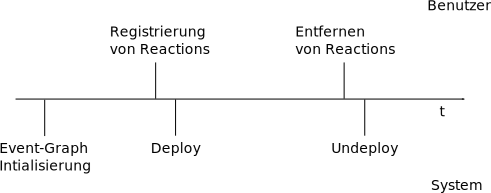
\includegraphics[width=0.7\textwidth]{graphics/EventNode-Lifecycle}
  \caption{Lifecycle eines EventNodes}
  \label{event_node_lifecycle}
\end{center}
\end{figure}


Es gibt, wie in Abb. \ref{interval_events_structure} zwei Klassen von
Interval-Event-Nodes: BetweenEvents und ExecutionEvents. BetweenEvents sind vom
Auftreten des StartEvents bis zum Auftreten des ersten End-Events aktiv, wenn
eine Reaction registiert wurde. Das Execution-Event dient dazu, die Ausf"uhrung
einer Funktion zu protokollieren. Wenn das Execution-Event eine Funktion
"uberwachen soll, dann instrumentiert der Compiler die Funktion so, dass ein
Before-Event beim Betreten der Funktion und ein After-Event beim Verlassen der
Funktion ausgel"ost wird.

%\usepackage{graphics} is needed for \includegraphics
\begin{figure}[htp]
\begin{center}
  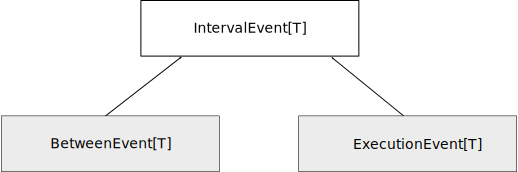
\includegraphics[width=0.5\textwidth]{graphics/interval_event_structure}
  \caption{Arten von Intervall-Events}
  \label{interval_events_structure}
\end{center}
\end{figure}


\subsection{Der Aufbau des Event-Graphen}
Mithilfe von Event-Nodes k"onnen mehrere Events zu komplexeren Events
zusammengefasst werden. So ist es beispielsweise m"oglich, alle Events einer
Filter-Bedingung zu unterziehen. Das resultierende Event wird nur dann
ausgel"ost, wenn ein zu filterndes Event auftritt dessen Filterbedingung zu true
auswertet. 

Der daraus resultierende Abh"anigkeitsgraph soll nachfolgend als Event-Graph
bezeichnet werden.

Intervall-Events k"onnen uneingeschr"ankt auch als Knoten im Event-Graph
vorkommen. Eine Liste der m"oglichen Filterfunktionen und die dazugeh"origen
Definitionen findet sich im Kapitel \ref{definitions}.

\subsection{Auswertung des Event-Graphen}

Bei der Auswertung eines Event-Graphen gibt es zwei m"oglichen Vorgehensweisen.
Zum einen kann Events sammeln, die bei Event-Graphen ankommen und dann
weiterleiten, wenn gewisse Bedingungen erf"ullt sind. Hierbei handelt es sich um
eine Push-basierte Implementierungen. Es werden n"amlich nur "Anderungen gepusht.

Beim Zweiten Ansatz werden keien "Andeurngen weitergeleitet. Stattdessen wird der
Event-Graph traversiert um herauszufinden, ob "Anderungen passiert sind. Dieser
Ansatz wird nachfolgend als pull-Basiert bezeichnet.

Bei gleichem Resultat haben beide Implementierungen verschiedene Vor- und
Nachteile. Nateilig beim Push-Basierten Ansatz ist die relativ hohe Komplexit"at
der Implementierung wenn Knoten im Event-Graph einen Zustand aufweisen.
Au\ss erdem ist es schwierig, ein deterministisches Verhalten sicherzustellen. Beim
Pull-basierten Ansatz stellt sich stattdessen die Frage, wie man den richtigen
Zeitpunkt f"ur einen Pull ermitteln kann. 

Die Implementierung im scala.events-Modul verwendet einen hybriden Ansatz um den
Event-Graphen auszuwerten. Die meisten Event-Knoten wurden Push-Basiert
implementiert. Eine Ausnahme stellt der Except-Knoten dar. Mit einem
Event-Knoten k"onnen verschiedene Events ausgeschlossen werden. Der Except-Zweig
des Event-Knotens wurde pull-basiert implementiert.

Betrachten wir nachfolgend zwei Beispiele um diese Vorgehensweise zu begr"unden:
\begin{eqnarray}
val \; e & = e1 \setminus (e2 || e3)\\
val \; e & = e1 \setminus (e1 || e3)
\end{eqnarray}

Der Event-Graph des Push-basierten Ansatzes ist in
Abb\ref{push_based_event_graph} zu sehen.

%\usepackage{graphics} is needed for \includegraphics
\begin{figure}[htp]
\centering
\subfigure[Push basierter Event-Gaph] {
  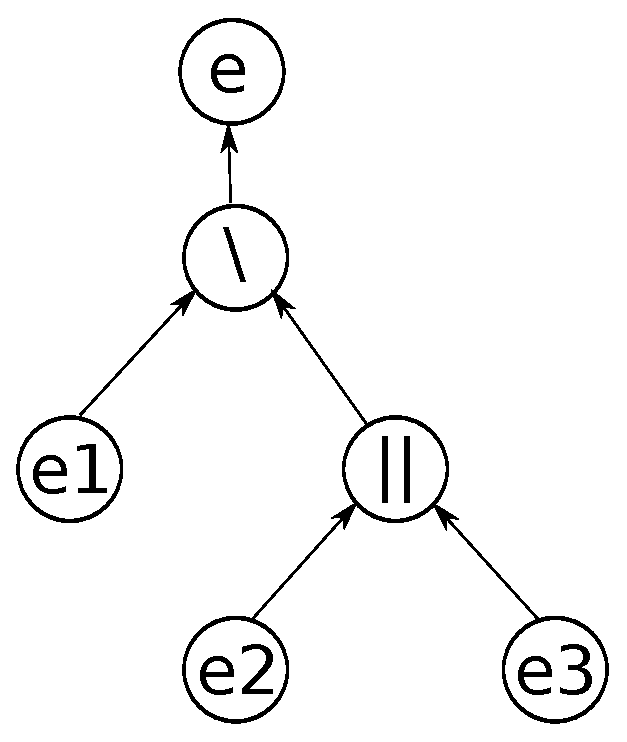
\includegraphics[width=0.3\textwidth]{graphics/event_node_except_push}
  \label{push_based_event_graph}
}
\subfigure[Push/Pull basierter Event-Graph] {
  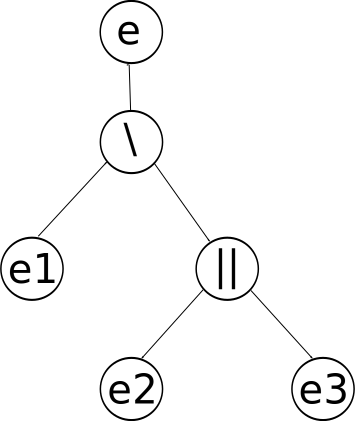
\includegraphics[width=0.3\textwidth]{graphics/event_node_except_pull}
  \label{pull_based_event_graph}
}
\caption{Event-Graphen f"ur das Beispiel 1}
\end{figure}

\begin{figure}[htp]
\centering
\subfigure[Push basierter Event-Gaph] {
  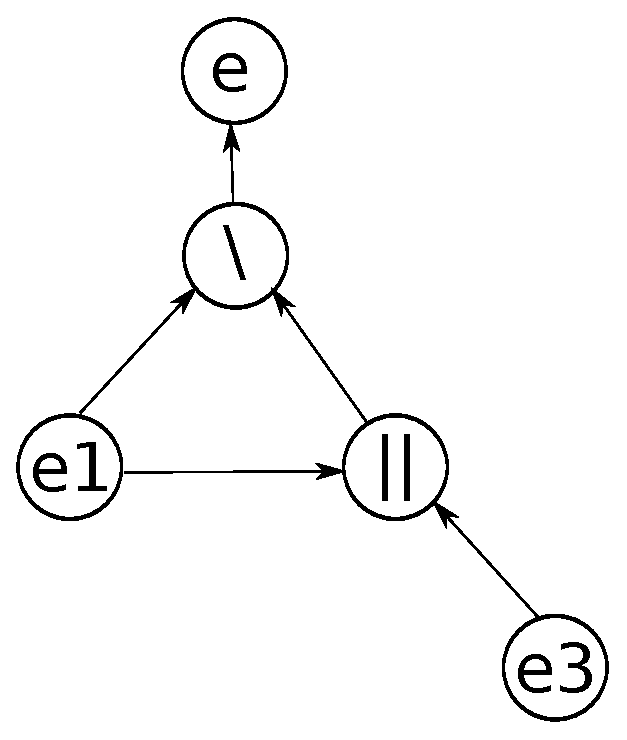
\includegraphics[width=0.3\textwidth]{graphics/event_node_except2_push}
  \label{failing_push_based_event_graph}
}
\subfigure[Push/Pull basierter Event-Graph] {
  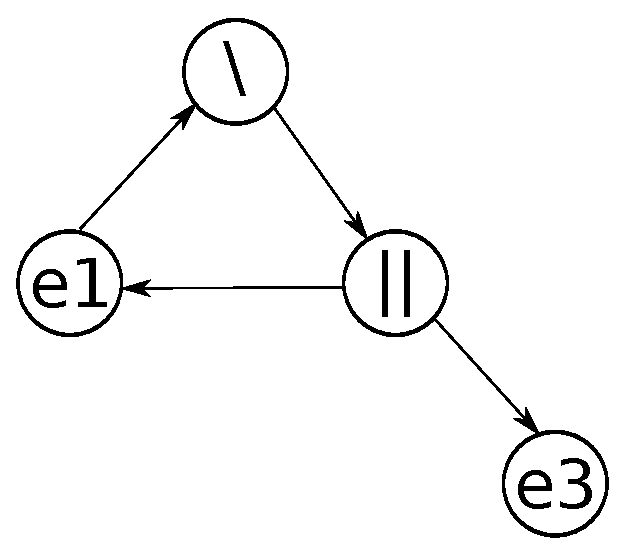
\includegraphics[width=0.3\textwidth]{graphics/event_node_except2_pull}
  \label{working_pull_based_event_graph}
}
\caption{Event-Graphen f"ur das Beispiel 2}
\end{figure}


\subsubsection{Einschr"ankungen der Implementierung}
In einem Event-Graph k"onnen nicht EventNodeRef oder EventNodeExists in einem
Pfad zusammen mit EventNodeExcept verwendet werden, da dies m"oglicherweise zu
nicht korrekten Ergebnissen f"uhren w"urde.

Beim EventNodeExcept kann ein Except-Event empfangen werden, der das Entfernen
von Reactions ausl"ost. Die sorgt m"oglicherweise f"ur Inkonsistenzen
bei Vorg"angerknoten im Event-Graphen, wenn sich die Reaction des Except-Knotens
vor der Reaction eines anderen Knotens in der ReactionListe befindet.
Daher muss im Falle eines Except-Events immer ein Undeploy und ein Deploy
ausgef"uhrt  werden, um die ge"anderten Reactions weiterzupropagieren.

Dies funktioniert allerdings nicht mehr l"anger mit EventNodeRef oder
EventNodeExists, dieses die Reihenfolge von Reactions ver"andern k"onnen.
